\chapter{基础CPU设计实现}\label{chap:03-base-cpu}

\section{EULA Core 简介}\label{sec:03-base-cpu-001}

EulaCore 是一个 9 级流水顺序单发射处理器，可启用分支预测器和 L1 Cache，支持 LoongArch32 Reduced 指令集中除浮点指令外的全部功能，使用 Chisel3 硬件描述语言实现。

EulaCore 的整体结构如下图所示：

\begin{figure}[htbp]
  \centering
  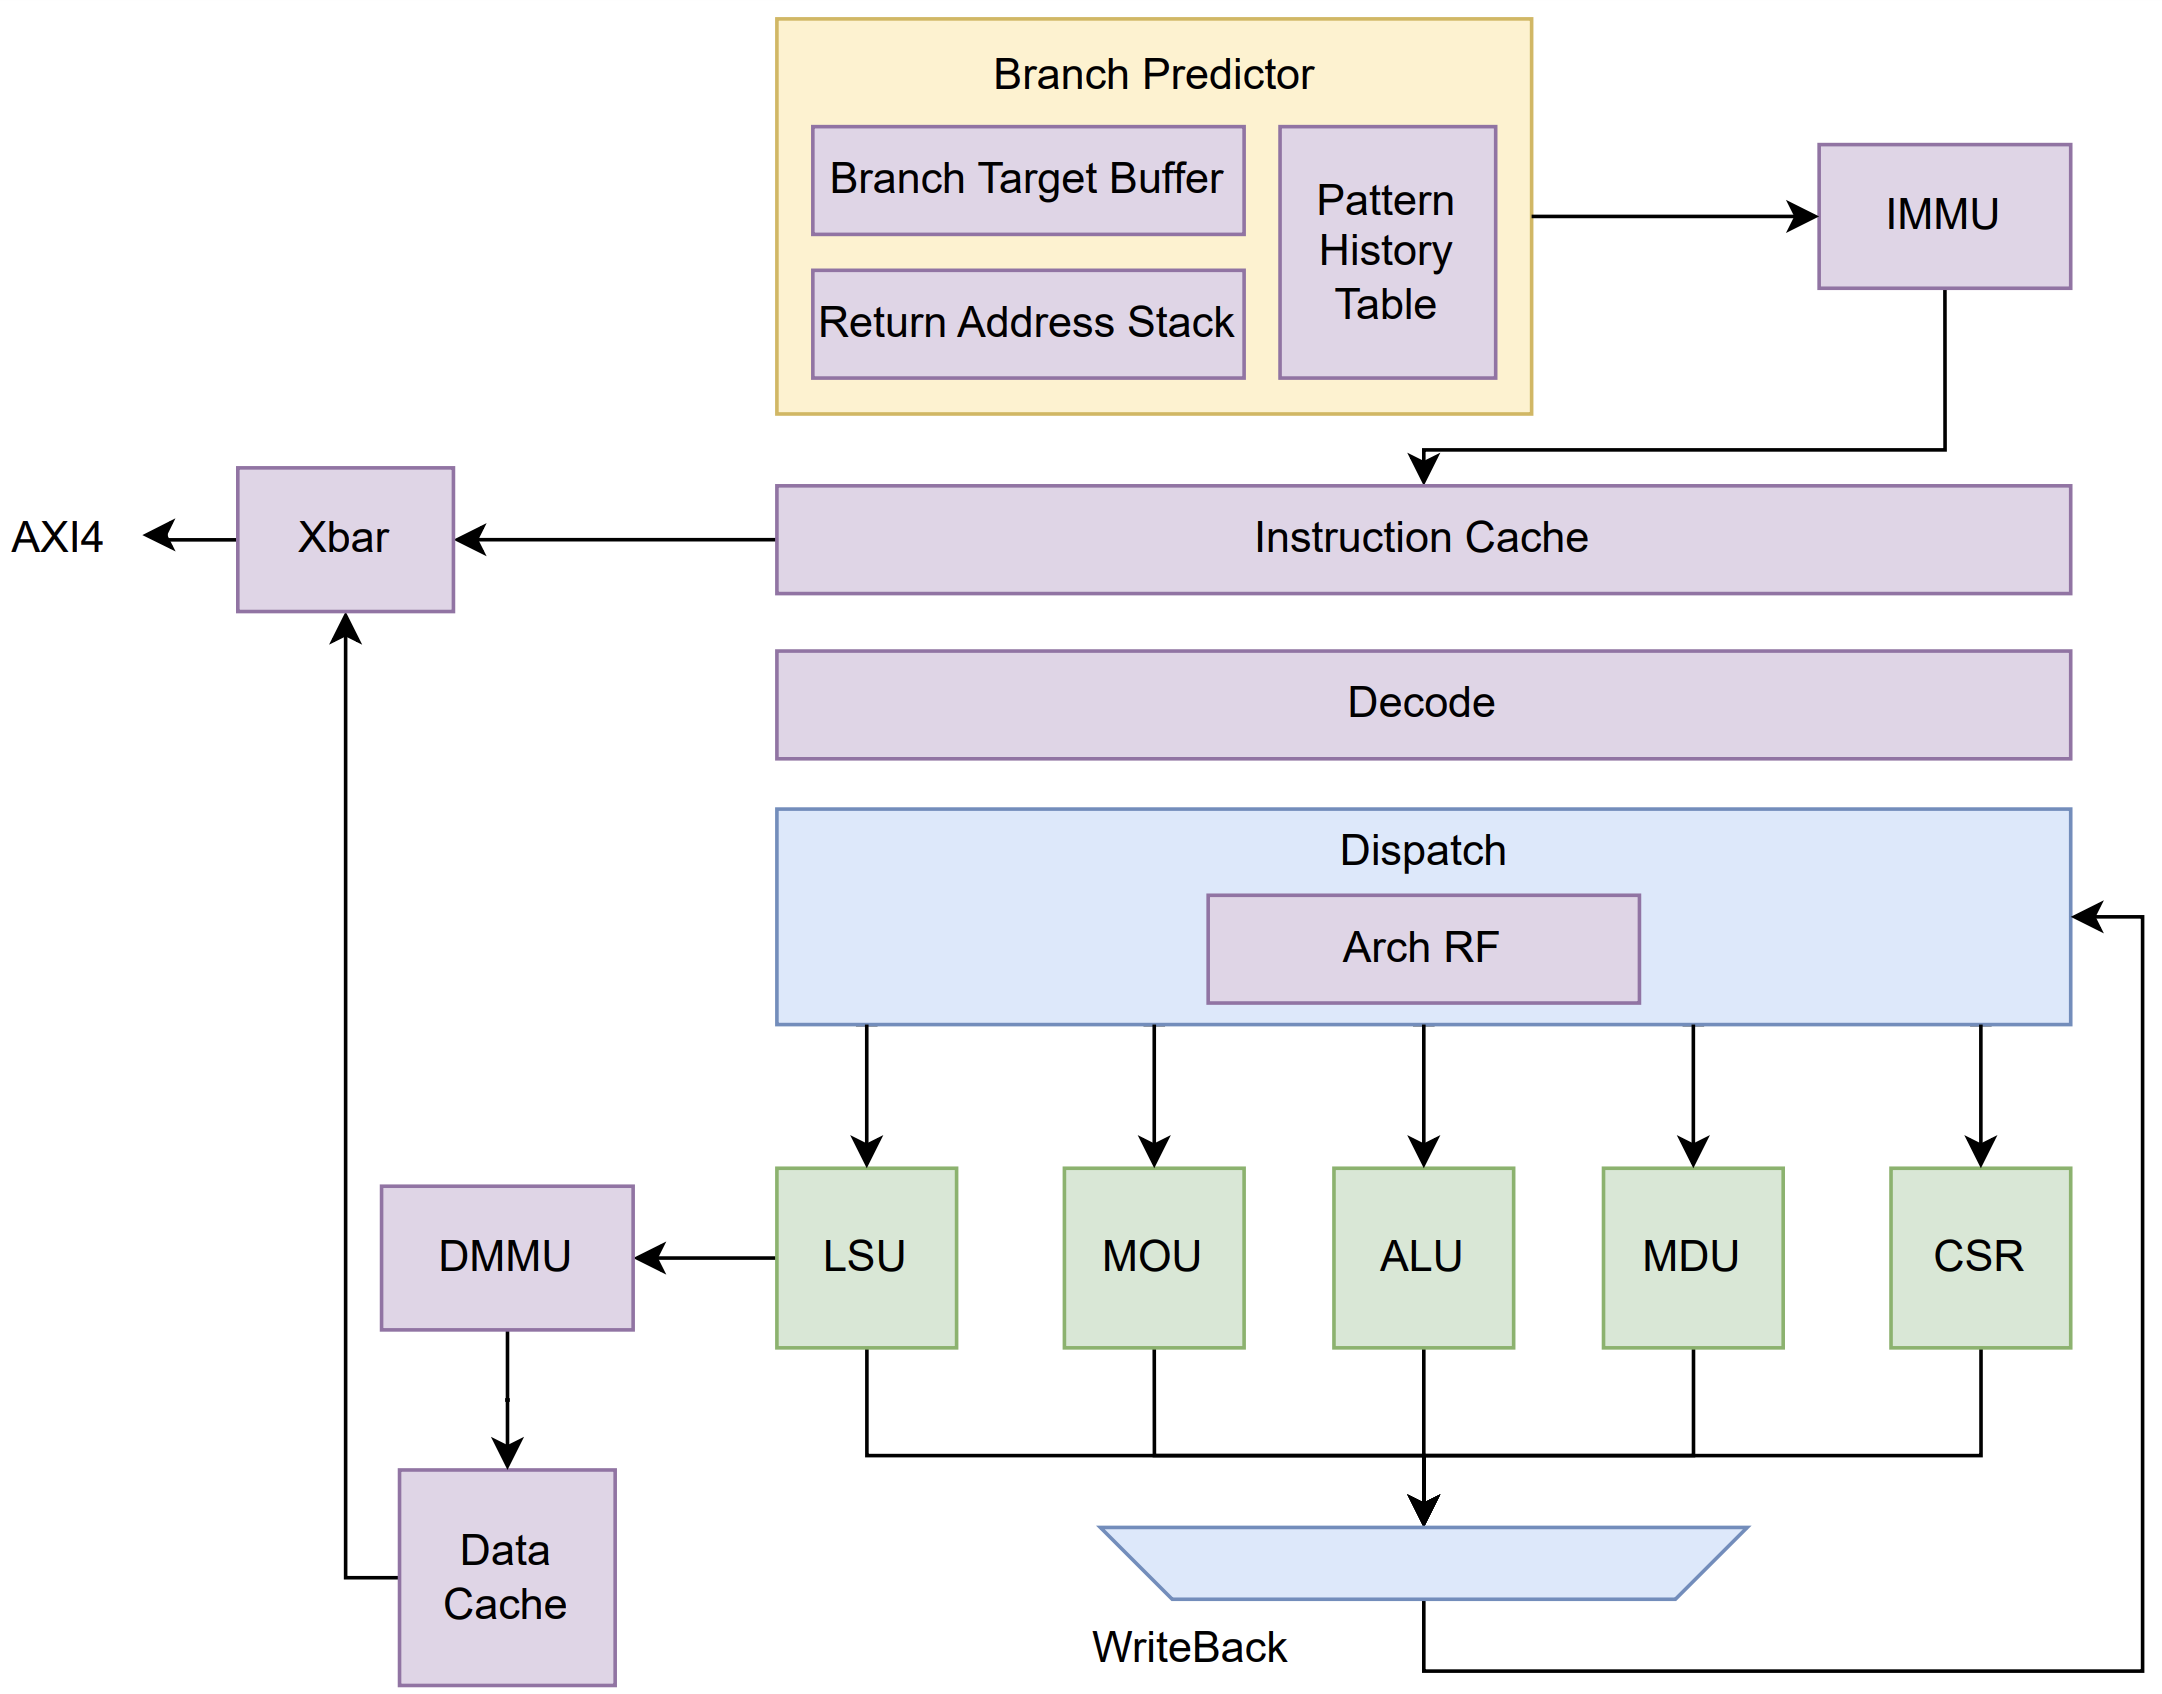
\includegraphics[width=1.0\linewidth]{assets/03/eula-arch.png}
  \caption{EULA Core架构图}
  \label{fig:03-eula-arch}
\end{figure}

分支预测单元提供对下一条指令 pc 的预测，预测 pc 经过 IMMU 转换为物理地址送入指令缓存进行查找，由指令缓存阻塞式处理缓存缺失，并返回指令送入 Decode 阶段进行译码。译码后的指令进入分派单元，并读寄存器堆。若指令所需的源操作数均已准备好，并且将被发射到的功能单元空闲，则指令会被发射到对应的功能单元执行。在功能单元执行完毕后，指令进入提交阶段，将结果写入寄存器堆。目前 EulaCore 使用计分板跟踪指令之间的相关性，全部流水线之间使用 valid-ready 双向握手机制。

下面对 EulaCore 中的一些重要模块进行分别介绍：

\subsection{分支预测模块}\label{sec:03-base-cpu-002}

分支预测器的结构如图所示：

\begin{figure}[htbp]
  \centering
  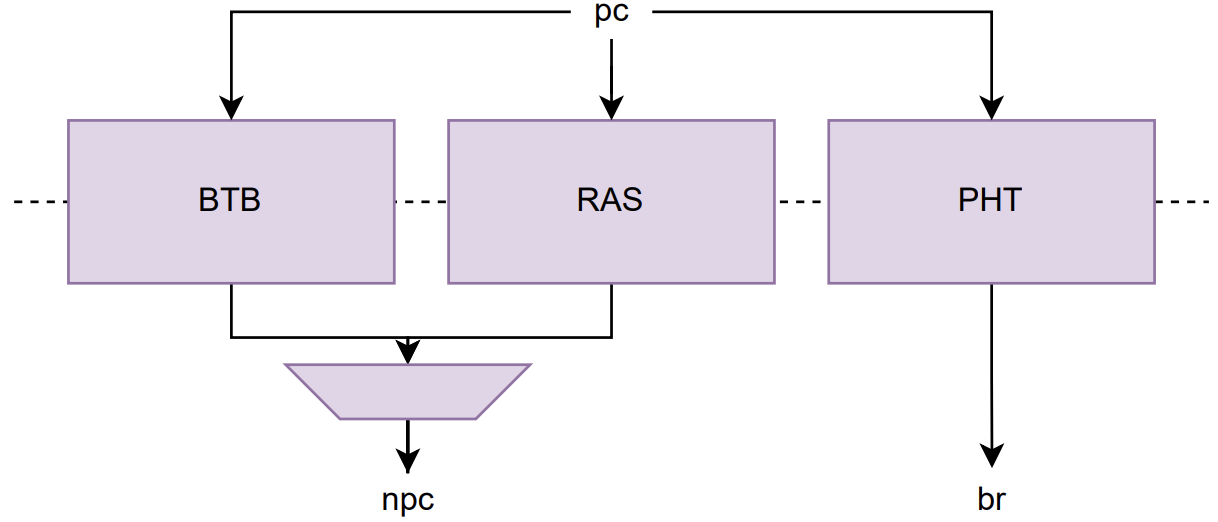
\includegraphics[width=0.5\linewidth]{assets/03/bpu-arch.png}
  \caption{分支预测模块结构}
  \label{fig:03-eula-bpu-arch}
\end{figure}

分支预测器通过综合考虑分支目标缓冲器 (Branch Target Buffer, BTB)、模式历史表(Pattern History Table, PHT) 和返回地址栈 (Return Address Stack, RAS) 对不同类型的转移指令做出快速的预测。

BTB,RAS,PHT 均使用单端口 SRAM 实现（FPGA 上会综合为 BRAM），采用硬件初始化。

BTB 中缓存了跳转指令的地址高位信息、跳转目标、指令类型等信息。在做分支预测时会用取指 PC 索引 BTB 表项，如果 PC 高位与读到的 BTB 表项的标签匹配则认为 BTB 命中，再根据 BTB 中记录的指令类型判断跳转方向和跳转目标。如果类型为条件分支指令，则需要访问模式历史表 (PHT) 来判断是否跳转; 如果类型为返回指令，则选择返回地址栈(RAS) 的栈顶内容作为跳转目标; 如果类型为直接或间接跳转指令，则选择 BTB 中记录的跳转目标。

\begin{itemize}
\item
  条件分支类指令：BEQ,BNE,BLT,BGE,BLTU,BGEU
\item
  直接跳转类指令：B
\item
  间接跳转类指令：BL，rd 不为 0 或 rj 不为 1 的 JIRL
\item
  返回指令：rd 为 0 且 rj 为 1 的 JIRL
\item
  函数调用指令：BL
\end{itemize}

PHT 的每一项都是一个两位饱和计数器，计数器的内容指示了强跳转、弱跳转、弱不跳转、强不跳转四种分支指令可能所处的状态，该两位计数器的高位则指示了分支预测的方向。

后端每执行一条函数调用指令 (BL) 或函数返回指令 (rd 为 0 且 rj 为 1 的 JIRL), 也会将相关信息传给分支预测器。如果该指令是 call 指令，则计算返回地址并写入 RAS 栈顶; 如果该指令是 ret 指令，则将 RAS 的栈顶弹出。

\subsection{译码模块设计}\label{sec:03-base-cpu-003}

译码模块根据指令码生成后端执行所需的一系列控制信号，信号名称与含义如下表所示：

\begin{longtable}[]{@{}
  >{\raggedright\arraybackslash}p{(\linewidth - 4\tabcolsep) * \real{0.0851}}
  >{\raggedright\arraybackslash}p{(\linewidth - 4\tabcolsep) * \real{0.5319}}
  >{\raggedright\arraybackslash}p{(\linewidth - 4\tabcolsep) * \real{0.3830}}@{}}
\toprule\noalign{}
\begin{minipage}[b]{\linewidth}\raggedright
信号名
\end{minipage} & \begin{minipage}[b]{\linewidth}\raggedright
含义
\end{minipage} & \begin{minipage}[b]{\linewidth}\raggedright
备注
\end{minipage} \\
\midrule\noalign{}
\endhead
\bottomrule\noalign{}
\endlastfoot
src1Type & 指令源操作数 1 的类型 & 可为 imm 或 reg，若为 imm，则在分派与发射阶段不考虑寄存器相关性 \\
src2Type & 指令源操作数 2 的类型 & 可为 imm 或 reg \\
fuType & 指令功能单元类型 & 可为 lsu，alu，mdu，mou，csr \\
fuOpType & 功能单元操作码 & \\
rfSrc1 & 源操作数 1 的寄存器堆编号 & 对应 LA32r 指令的 rj \\
rfSrc2 & 源操作数 2 的寄存器堆编号 & 一般对应 LA32r 指令的 rk，若为分支指令或 store 类指令，则为 rd \\
rfWen & 指令是否要写寄存器 & \\
rfDest & 指令写入的目的寄存器号 & \\
imm & 指令立即数 & \\
\end{longtable}

EulaCore 基于 chisel 提供的 BitPat API 实现了较为简洁的译码过程，指令编码通过BitPat 存储，指令控制信号单独存储，提高了可读性，以下为一个示例：

% 代码语言：BookScala
\begin{CodeBlock}[language=BookScala]
object LA32R_MOUInstr extends HasLa32rInstrType with HasEulaCoreParameter {

  def DBAR      = BitPat("b0 0 1 1 1 0 0 0 0 1 1 1 0 0 1 0 0_???????????????")
  def IBAR      = BitPat("b0 0 1 1 1 0 0 0 0 1 1 1 0 0 1 0 1_???????????????")

  val table = Array(// (instrType, FuType, FuOpType, isrfWen)
    DBAR      -> List(InstrCODE15, FuType.mou, La32rMOUOpType.dbar, false.B),
    IBAR      -> List(InstrCODE15, FuType.mou, La32rMOUOpType.ibar, false.B),
  )
}
\end{CodeBlock}

\subsection{访存单元（LSU）设计}\label{sec:03-base-cpu-004}

LSU 模块负责与数据缓存交互，处理 load 与 store 类指令，其主体是一个状态机：

\begin{figure}[htbp]
  \centering
  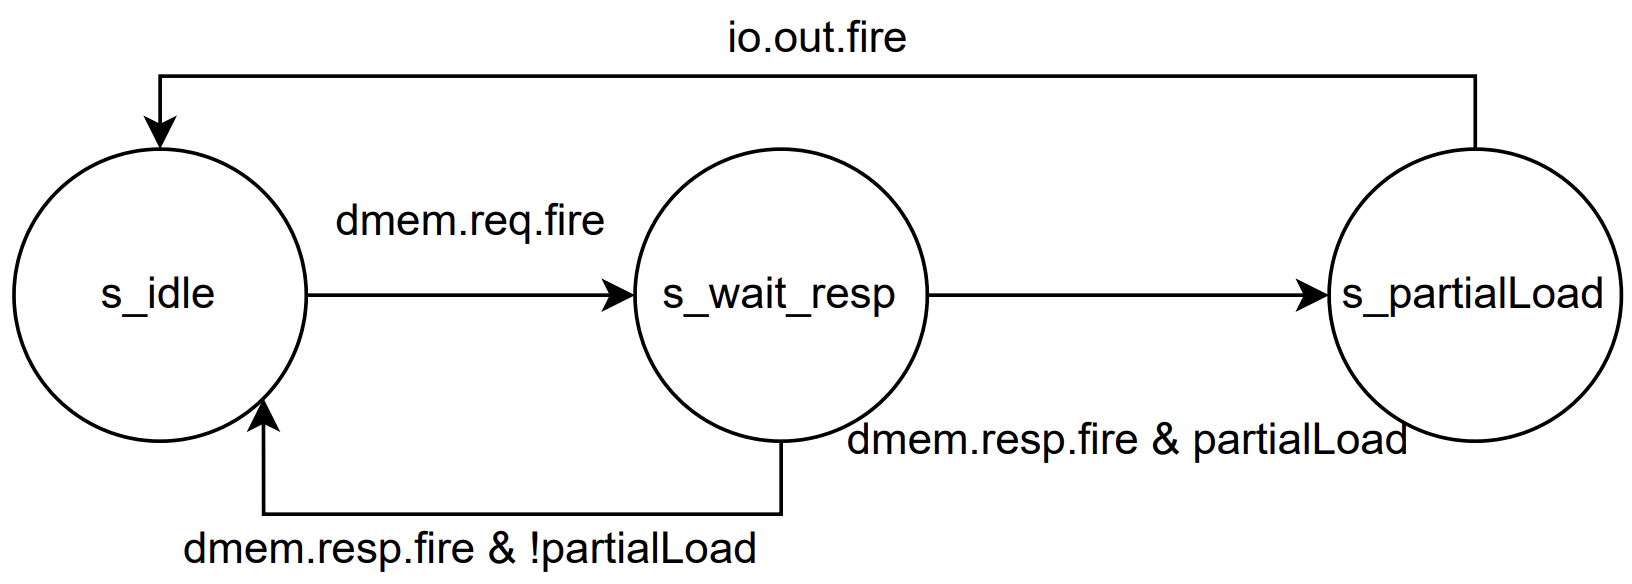
\includegraphics[width=0.5\linewidth]{assets/03/lsu-state.png}
  \caption{LSU状态机}
  \label{fig:03-lsu-state}
\end{figure}

访存指令来到 LSU 后会向 DCache 发出请求，若与 DCache 握手成功则状态机从 s\_idle转到 s\_wait\_resp 状态，等待 DCache 返回读数据或写响应信号。

如果是 ld.w 指令，则数据从 DCache 返回后 LSU 将直接将指令放行至随后的流水级，如果是 ld.h，ld.b，ld.hu，ld.bu，则在数据返回后状态机会转移至 s\_partialLoad 状态，进行返回数据切分后再将指令放行。DCache 是一个 3 级流水线结构，因此在命中情况下，store 类指令或 ld.w 指令在 LSU 需要经历 3 个周期，ld.h，ld.b，ld.hu，ld.bu 在 LSU 需要经历 4 个周期。

如果在访存过程中触发了 tlb 异常，或者访存地址触发了地址非对齐异常，那么 LSU 会将指令转发给 CSR 单元，由 CSR 单元进行异常处理。

\subsection{访存定序单元（MOU）设计}\label{sec:03-base-cpu-005}

MOU 模块负责访存定序，ibar 指令与 dbar 指令由 MOU 单元执行。

EulaCore 并没有乱序执行 load/store 指令，因此 dbar指令视作 nop 处理。

ibar 指令需要保证 ibar 指令后的取指一定能够观察到 ibar 指令前所有 store 操作的执行效果，对此 EulaCore 的实现方式是将 dcache 全部无效并写回内存，然后全部无效icache。这个过程由 MOU 的状态机控制：

\begin{figure}[htbp]
  \centering
  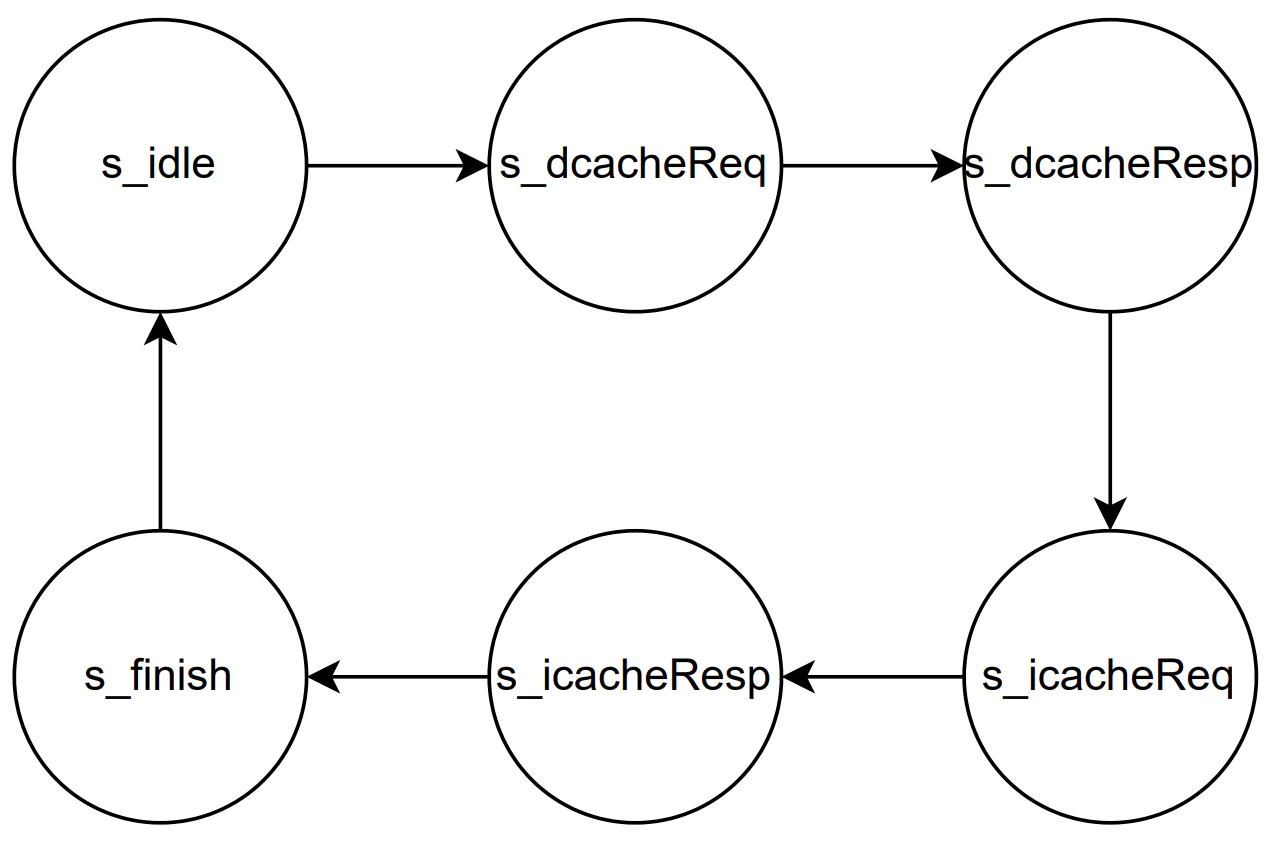
\includegraphics[width=0.5\linewidth]{assets/03/mou-state.png}
  \caption{MOU状态机}
  \label{fig:03-mou-state}
\end{figure}

当 ibar 或 dbar 提交时，处理器会冲刷流水线并重定向至 ibar 或 dbar 的 pc + 4 的位置重新取指并执行。

\subsection{CSR 模块设计}\label{sec:03-base-cpu-006}

CSR 模块中包含所有指令集定义的 CSR 寄存器，它负责执行所有特权指令，并产生异常中断。

在 CSR 单元中，EulaCore 大量地使用了 BoringUtils 这一 Chisel 内置类来进行飞线，这是因为很多其他的功能部件需要从 CSR 中获取到当前系统状态来实现相应功能 (比如LSU, MMU 等)。

另外需要注意的是，TLBSRCH，TLBRD 指令对 TLB 的访问与 TLB 进行虚拟地址到物理地址的转换过程类似，当前 TLB 为纯组合逻辑，为了避免在 TLB 模块中除了一般地址转换的电路外，增加对 TLBSRCH,TLBRD 指令查找 TLB 表项的电路支持从而造成 TLB 的时序压力过大，在 CSR 中另外实例化了一个 TLB，用于 TLBSRCH 与 TLBRD 指令的查找需求。

另外，HIT 类 CACOP 指令也可能需要查找 TLB 进行地址转换，因此在 CSR 中又另外实例化了一个 TLB 用于 HIT 类 CACOP 指令的地址转换需求。因此，当前 EulaCore 中一共有 4 个 TLB，IMMU,DMMU 中各一个，CSR 中有两个，这 4 个 TLB 的内容完全一致。

\section{流水线结构}\label{sec:03-base-cpu-007}

在 EULA Core 中，前后端通过 PipelineVector2Connect 模块相连，理论上支持双发射。

PipelineVector2Connect模块内部实现了一个 FIFO，前端译码完成后可向该 FIFO 中写入指令信息，后端再从该 FIFO 中取出指令信息，FIFO 大小支持自定义。

% 代码语言：BookScala
\begin{CodeBlock}[language=BookScala]
object PipelineVector2Connect {
  def apply[T <: Data](gen: T, in1: DecoupledIO[T], in2: DecoupledIO[T], out1: DecoupledIO[T], out2: DecoupledIO[T], flush: Bool, bufferSize: Int) = {

    //ring buffer
    val dataBuffer = RegInit(VecInit(Seq.fill(bufferSize)(0.U.asTypeOf(gen))))
    val ringBufferHead = RegInit(0.U(log2Up(bufferSize).W))
    val ringBufferTail = RegInit(0.U(log2Up(bufferSize).W))
    val ringBufferEmpty = ringBufferHead === ringBufferTail
    val ringBufferAllowin = (0 to 1).map(i => (ringBufferHead + (i+1).U) =/= ringBufferTail).foldRight(true.B)((sum,i)=>sum&i)
    
    //enqueue
    val needEnqueue = Wire(Vec(2, Bool()))
    needEnqueue(0) := in1.valid
    needEnqueue(1) := in2.valid

    val enqueueSize = needEnqueue(0).asUInt()+&needEnqueue(1).asUInt() // count(true) in needEnqueue
    val enqueueFire = (0 to 1).map(i => enqueueSize >= (i+1).U)

    val wen = in1.fire() || in2.fire() // i.e. ringBufferAllowin && in.valid
    when(wen){
        when(enqueueFire(0)){dataBuffer(0.U + ringBufferHead) := Mux(needEnqueue(0), in1.bits, in2.bits)}
        when(enqueueFire(1)){dataBuffer(1.U + ringBufferHead) := in2.bits}
        ringBufferHead := ringBufferHead + enqueueSize
    }

    in1.ready := ringBufferAllowin || !in1.valid
    in2.ready := ringBufferAllowin || !in2.valid

    //dequeue socket 1
    val deq1_StartIndex = ringBufferTail
    out1.bits := dataBuffer(deq1_StartIndex)
    out1.valid := ringBufferHead =/= deq1_StartIndex

    //dequeue socket 2
    val deq2_StartIndex = ringBufferTail + 1.U
    out2.bits := dataBuffer(deq2_StartIndex)
    out2.valid := ringBufferHead =/= deq2_StartIndex && out1.valid

    //dequeue control
    val dequeueSize = out1.fire().asUInt() +& out2.fire().asUInt
    val dequeueFire = dequeueSize > 0.U
    when(dequeueFire){
        ringBufferTail := ringBufferTail + dequeueSize;
    }

    //flush control
    when(flush){
        ringBufferHead := 0.U
        ringBufferTail := 0.U
    }

  }
}
\end{CodeBlock}

前端和后端内部流水结构如前面所述。

\section{处理数据相关性}\label{sec:03-base-cpu-008}

在 EULA Core 中，定义了 isDepend 函数用于判断各流水级之间的数据冲突：

% 代码语言：BookScala
\begin{CodeBlock}[language=BookScala]
  def isDepend(rfSrc: UInt, rfDest: UInt, wen: Bool): Bool = (rfSrc =/= 0.U) && (rfSrc === rfDest) && wen

  val forwardRfWen = io.forward.wb.rfWen && io.forward.valid
  val dontForward1 = (io.forward.fuType =/= FuType.alu) && (io.forward.fuType =/= FuType.lsu)
  val src1DependEX = isDepend(rfSrc1, io.forward.wb.rfDest, forwardRfWen)
  val src2DependEX = isDepend(rfSrc2, io.forward.wb.rfDest, forwardRfWen)
  val src1DependWB = isDepend(rfSrc1, io.wb.rfDest, io.wb.rfWen)
  val src2DependWB = isDepend(rfSrc2, io.wb.rfDest, io.wb.rfWen)
\end{CodeBlock}

以 src1DependEX 为例，如果发生了数据依赖，则会进行数据选择：

% 代码语言：BookScala
\begin{CodeBlock}[language=BookScala]
val src1ForwardNextCycle = src1DependEX && !dontForward1
val src2ForwardNextCycle = src2DependEX && !dontForward1
val src1Forward = src1DependWB && Mux(dontForward1, !src1DependEX, true.B)
val src2Forward = src2DependWB && Mux(dontForward1, !src2DependEX, true.B)
\end{CodeBlock}

而操作数的状态可以通过 src1Ready 和 src2Ready 表明，如果该信号为低电平，则握手信号的 valid 信号 置低，此时后级不会接受此级传入的数据。

% 代码语言：BookScala
\begin{CodeBlock}[language=BookScala]
io.out.valid := io.in(0).valid && src1Ready && src2Ready
\end{CodeBlock}

\section{旁路结构}\label{sec:03-base-cpu-009}

在 EULA Core 中，写回级的数据通过 ForwardIO 向前进行旁路传递。

% 代码语言：BookScala
\begin{CodeBlock}[language=BookScala]
class ForwardIO extends EulaCoreBundle {
  val valid = Output(Bool())
  val wb = new WriteBackIO
  val fuType = Output(FuType())
}
\end{CodeBlock}

然后，在 发射级（ISU）和执行级（EXU），会传入 ForwardIO 信号获取旁路数据。
